\documentclass{standalone}
\usepackage{tikz}
\usetikzlibrary{patterns, positioning}

\begin{document}
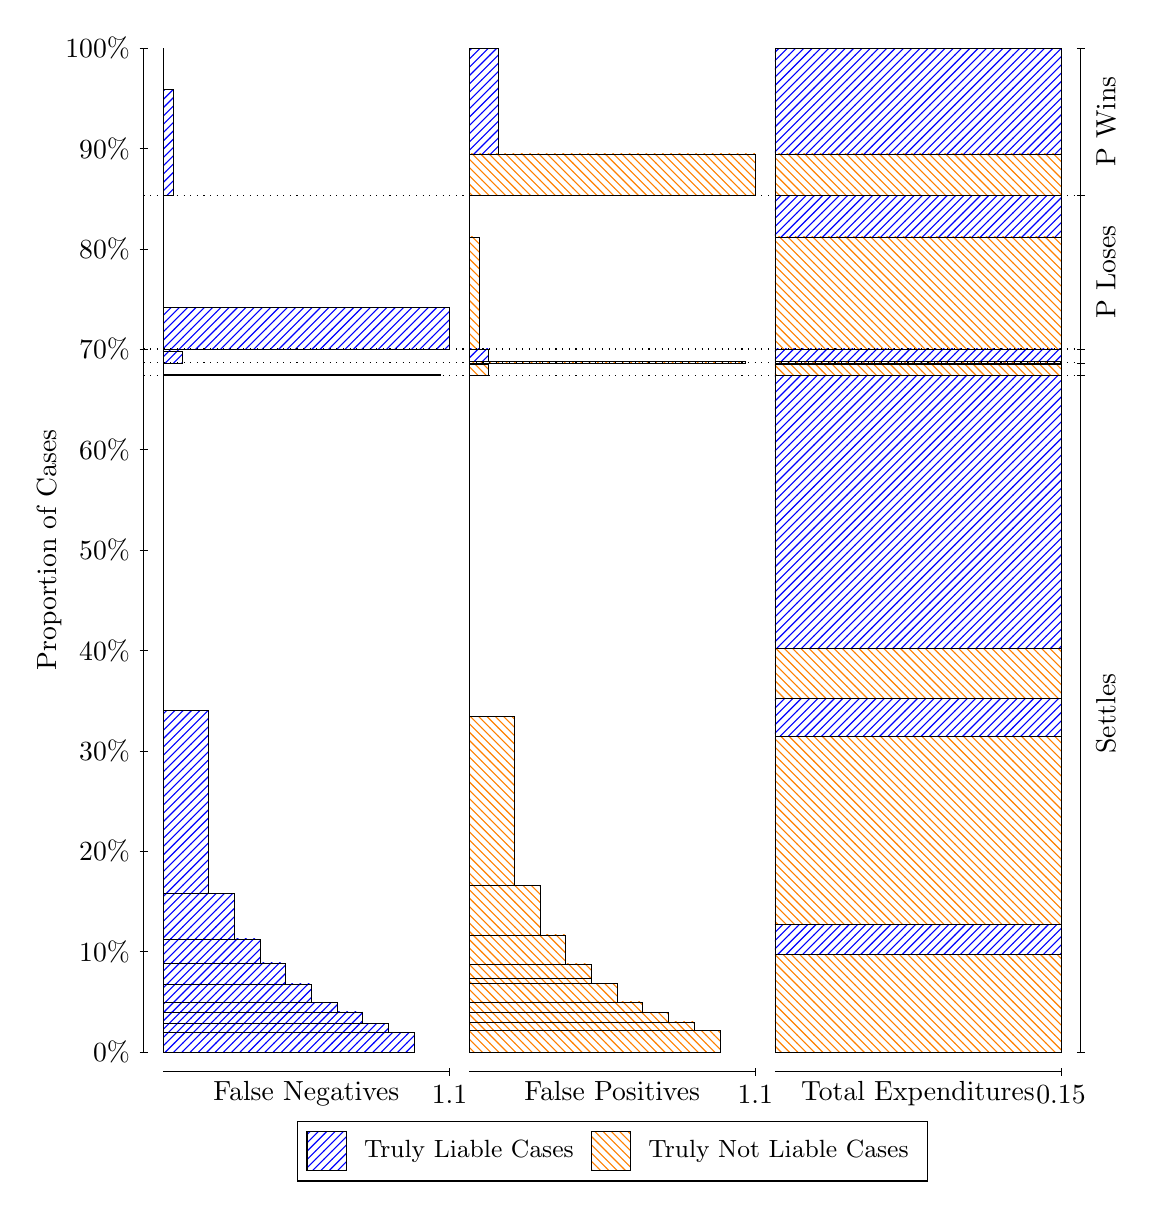
\begin{tikzpicture}
\draw[black, very thin] (1.5,1.75) -- (1.5,14.5);
\node[rotate=90, anchor=center] at (0.3, 8.125) {Proportion of Cases};
\draw[black, very thin] (1.45,1.75) -- (1.55,1.75);
\node[anchor=east] at (1.45, 1.75) {0\%};
\draw[black, very thin] (1.45,3.025) -- (1.55,3.025);
\node[anchor=east] at (1.45, 3.025) {10\%};
\draw[black, very thin] (1.45,4.3) -- (1.55,4.3);
\node[anchor=east] at (1.45, 4.3) {20\%};
\draw[black, very thin] (1.45,5.575) -- (1.55,5.575);
\node[anchor=east] at (1.45, 5.575) {30\%};
\draw[black, very thin] (1.45,6.85) -- (1.55,6.85);
\node[anchor=east] at (1.45, 6.85) {40\%};
\draw[black, very thin] (1.45,8.125) -- (1.55,8.125);
\node[anchor=east] at (1.45, 8.125) {50\%};
\draw[black, very thin] (1.45,9.4) -- (1.55,9.4);
\node[anchor=east] at (1.45, 9.4) {60\%};
\draw[black, very thin] (1.45,10.675) -- (1.55,10.675);
\node[anchor=east] at (1.45, 10.675) {70\%};
\draw[black, very thin] (1.45,11.95) -- (1.55,11.95);
\node[anchor=east] at (1.45, 11.95) {80\%};
\draw[black, very thin] (1.45,13.225) -- (1.55,13.225);
\node[anchor=east] at (1.45, 13.225) {90\%};
\draw[black, very thin] (1.45,14.5) -- (1.55,14.5);
\node[anchor=east] at (1.45, 14.5) {100\%};

\draw[black, very thin] (13.4,1.75) -- (13.4,14.5);
\draw[black, very thin] (13.35,1.75) -- (13.45,1.75);
\node[anchor=west] at (13.35, 1.75) {};
\draw[black, very thin] (13.35,10.346) -- (13.45,10.346);
\node[anchor=west] at (13.35, 10.346) {};
\draw[black, very thin] (13.35,10.502) -- (13.45,10.502);
\node[anchor=west] at (13.35, 10.502) {};
\draw[black, very thin] (13.35,10.678) -- (13.45,10.678);
\node[anchor=west] at (13.35, 10.678) {};
\draw[black, very thin] (13.35,12.629) -- (13.45,12.629);
\node[anchor=west] at (13.35, 12.629) {};
\draw[black, very thin] (13.35,14.5) -- (13.45,14.5);
\node[anchor=west] at (13.35, 14.5) {};

\draw[black, very thin, pattern color=blue, pattern=north east lines] (1.75,1.75) rectangle (4.9343,1.9979);
\draw[black, very thin, pattern color=blue, pattern=north east lines] (1.75,1.9979) rectangle (4.6077,2.118);
\draw[black, very thin, pattern color=blue, pattern=north east lines] (1.75,2.118) rectangle (4.2811,2.2586);
\draw[black, very thin, pattern color=blue, pattern=north east lines] (1.75,2.2586) rectangle (3.9545,2.3778);
\draw[black, very thin, pattern color=blue, pattern=north east lines] (1.75,2.3778) rectangle (3.6279,2.6139);
\draw[black, very thin, pattern color=blue, pattern=north east lines] (1.75,2.6139) rectangle (3.3013,2.8824);
\draw[black, very thin, pattern color=blue, pattern=north east lines] (1.75,2.8824) rectangle (2.9747,3.1872);
\draw[black, very thin, pattern color=blue, pattern=north east lines] (1.75,3.1872) rectangle (2.6481,3.7661);
\draw[black, very thin, pattern color=blue, pattern=north east lines] (1.75,3.7661) rectangle (2.3215,6.0874);
\draw[black, very thin, pattern color=orange, pattern=north west lines] (1.75,6.0874) rectangle (1.75,10.346);
\draw[black, very thin, pattern color=blue, pattern=north east lines] (1.75,10.346) rectangle (5.2609,10.36);
\draw[black, very thin, pattern color=orange, pattern=north west lines] (1.75,10.36) rectangle (1.75,10.502);
\draw[black, very thin, pattern color=blue, pattern=north east lines] (1.75,10.502) rectangle (1.9949,10.654);
\draw[black, very thin, pattern color=orange, pattern=north west lines] (1.75,10.654) rectangle (1.75,10.678);
\draw[black, very thin, pattern color=blue, pattern=north east lines] (1.75,10.678) rectangle (5.3833,11.205);
\draw[black, very thin, pattern color=orange, pattern=north west lines] (1.75,11.205) rectangle (1.75,12.629);
\draw[black, very thin, pattern color=blue, pattern=north east lines] (1.75,12.629) rectangle (1.8725,13.973);
\draw[black, very thin, pattern color=orange, pattern=north west lines] (1.75,13.973) rectangle (1.75,14.5);
\draw[black, very thin, pattern color=orange, pattern=north west lines] (5.6333,1.75) rectangle (8.8176,2.0202);
\draw[black, very thin, pattern color=orange, pattern=north west lines] (5.6333,2.0202) rectangle (8.491,2.1335);
\draw[black, very thin, pattern color=orange, pattern=north west lines] (5.6333,2.1335) rectangle (8.1644,2.2524);
\draw[black, very thin, pattern color=orange, pattern=north west lines] (5.6333,2.2524) rectangle (7.8378,2.3855);
\draw[black, very thin, pattern color=orange, pattern=north west lines] (5.6333,2.3855) rectangle (7.5112,2.6258);
\draw[black, very thin, pattern color=orange, pattern=north west lines] (5.6333,2.6258) rectangle (7.1846,2.6801);
\draw[black, very thin, pattern color=orange, pattern=north west lines] (5.6333,2.6801) rectangle (7.1846,2.8674);
\draw[black, very thin, pattern color=orange, pattern=north west lines] (5.6333,2.8674) rectangle (6.8581,3.2383);
\draw[black, very thin, pattern color=orange, pattern=north west lines] (5.6333,3.2383) rectangle (6.5315,3.8697);
\draw[black, very thin, pattern color=orange, pattern=north west lines] (5.6333,3.8697) rectangle (6.2049,6.0089);
\draw[black, very thin, pattern color=blue, pattern=north east lines] (5.6333,6.0089) rectangle (5.6333,10.346);
\draw[black, very thin, pattern color=orange, pattern=north west lines] (5.6333,10.346) rectangle (5.8783,10.488);
\draw[black, very thin, pattern color=blue, pattern=north east lines] (5.6333,10.488) rectangle (5.6333,10.502);
\draw[black, very thin, pattern color=orange, pattern=north west lines] (5.6333,10.502) rectangle (9.1442,10.525);
\draw[black, very thin, pattern color=blue, pattern=north east lines] (5.6333,10.525) rectangle (5.8783,10.678);
\draw[black, very thin, pattern color=orange, pattern=north west lines] (5.6333,10.678) rectangle (5.7558,12.102);
\draw[black, very thin, pattern color=blue, pattern=north east lines] (5.6333,12.102) rectangle (5.6333,12.629);
\draw[black, very thin, pattern color=orange, pattern=north west lines] (5.6333,12.629) rectangle (9.2667,13.156);
\draw[black, very thin, pattern color=blue, pattern=north east lines] (5.6333,13.156) rectangle (6.0007,14.5);
\draw[black, very thin, pattern color=orange, pattern=north west lines] (9.5167,1.75) rectangle (13.15,2.9939);
\draw[black, very thin, pattern color=blue, pattern=north east lines] (9.5167,2.9939) rectangle (13.15,3.3738);
\draw[black, very thin, pattern color=orange, pattern=north west lines] (9.5167,3.3738) rectangle (13.15,5.7534);
\draw[black, very thin, pattern color=blue, pattern=north east lines] (9.5167,5.7534) rectangle (13.15,6.2373);
\draw[black, very thin, pattern color=orange, pattern=north west lines] (9.5167,6.2373) rectangle (13.15,6.8728);
\draw[black, very thin, pattern color=blue, pattern=north east lines] (9.5167,6.8728) rectangle (13.15,10.346);
\draw[black, very thin, pattern color=orange, pattern=north west lines] (9.5167,10.346) rectangle (13.15,10.488);
\draw[black, very thin, pattern color=blue, pattern=north east lines] (9.5167,10.488) rectangle (13.15,10.502);
\draw[black, very thin, pattern color=orange, pattern=north west lines] (9.5167,10.502) rectangle (13.15,10.525);
\draw[black, very thin, pattern color=blue, pattern=north east lines] (9.5167,10.525) rectangle (13.15,10.678);
\draw[black, very thin, pattern color=orange, pattern=north west lines] (9.5167,10.678) rectangle (13.15,12.102);
\draw[black, very thin, pattern color=blue, pattern=north east lines] (9.5167,12.102) rectangle (13.15,12.629);
\draw[black, very thin, pattern color=orange, pattern=north west lines] (9.5167,12.629) rectangle (13.15,13.156);
\draw[black, very thin, pattern color=blue, pattern=north east lines] (9.5167,13.156) rectangle (13.15,14.5);
\draw[black, dotted] (1.5,10.346) -- (13.4,10.346);
\draw[black, dotted] (1.5,10.502) -- (13.4,10.502);
\draw[black, dotted] (1.5,10.678) -- (13.4,10.678);
\draw[black, dotted] (1.5,12.629) -- (13.4,12.629);
\draw[black, very thin] (1.75,1.5) -- (5.3833,1.5);
\node[anchor=north] at (3.5667, 1.5) {False Negatives};
\draw[black, very thin] (5.3833,1.45) -- (5.3833,1.55);
\node[anchor=north] at (5.3833, 1.45) {1.1};

\draw[black, very thin] (5.6333,1.5) -- (9.2667,1.5);
\node[anchor=north] at (7.45, 1.5) {False Positives};
\draw[black, very thin] (9.2667,1.45) -- (9.2667,1.55);
\node[anchor=north] at (9.2667, 1.45) {1.1};

\draw[black, very thin] (9.5167,1.5) -- (13.15,1.5);
\node[anchor=north] at (11.333, 1.5) {Total Expenditures};
\draw[black, very thin] (13.15,1.45) -- (13.15,1.55);
\node[anchor=north] at (13.15, 1.45) {0.15};

\node[black, centered, rotate=90] at (13.72, 6.0481) {Settles};


\node[black, centered, rotate=90] at (13.72, 11.653) {P Loses};
\node[black, centered, rotate=90] at (13.72, 13.565) {P Wins};

\draw (7.449999999999999,1.5) node[draw=none] (baseCoordinate) {};
\begin{scope}[align=center]
        \matrix[scale=0.5, draw=black, below=0.5cm of baseCoordinate, nodes={draw}, column sep=0.1cm]{
            \node[rectangle, draw, minimum width=0.5cm, minimum height=0.5cm, pattern=north east lines, pattern color=blue] {}; &
            \node[draw=none, font=\small] (B) {Truly Liable Cases}; &
            \node[rectangle, draw, minimum width=0.5cm, minimum height=0.5cm, pattern=north west lines, pattern color=orange] {}; &
            \node[draw=none, font=\small] (B) {Truly Not Liable Cases}; \\
            };
\end{scope}

\end{tikzpicture}
\end{document}